\documentclass[]{beamer}
\mode<presentation>{
  %% \usetheme[compress]{Berlin}
}
%% packages
\usepackage{zhspacing}
\zhspacing
\usepackage{graphics}
\usepackage{listings}
\lstset{
  basicstyle=\ttfamily\tiny,
  numbers=left
}
\usepackage{tabularx}
\usepackage{booktabs}
%% meta info
\title{Pregel: Large-Scale Graph Processing}
%% \subtitle{}
\author[SuXing~pysuxing@gmail.com]{SuXing}
\institute{TOW}
\date{\today}

\setbeamercolor{footcolor}{fg=blue,bg=white} % 设置字体和背景颜色
\setbeamertemplate{footline}{%
  \leavevmode%
  \hbox{%
    \begin{beamercolorbox}[wd=.126\paperwidth,ht=2.25ex,dp=1ex,right]{footcolor}%      
       \insertframenumber{} / \inserttotalframenumber\hspace*{5ex}
    \end{beamercolorbox}}%
  \vskip0pt%
}

%% slides
\begin{document}
\setlength{\parindent}{0pt}

\frame{\titlepage}
\frame{\tableofcontents}

\section{Large-Scale Graph}
\frame{\tableofcontents[currentsection]}

\begin{frame}
  \frametitle{How Large?}
  How large we mean saying \alert{Large-scale} Graph?
  \begin{itemize}
    \item billions of vertices
    \item tens of billions of edges or more
  \end{itemize}

  \pause
  Often only solvable in distributed computing systems (MPP or clusters)
\end{frame}

\begin{frame}
  \frametitle{Realworld Applications}
  Almost all complex systems are abstracted to large-scale graphs
  \begin{itemize}
    \item world-wide-web
    \item socail network
  \end{itemize}
\end{frame}

\begin{frame}
  \frametitle{Challenges in Large-Scale Graph Processing}
  These large-scale graphs have properties bringing nightmare to
  traditional distributed computing techniques
  \begin{itemize}
    \item low data locality
    \item low comp./comm. ratio
    \item dynamic load distribution
  \end{itemize}

  \pause
  Besides the performance issue, programming graph algorithms on distributed systems
  is difficult and error prone
\end{frame}

\section{Pregel}
\frame{\tableofcontents[currentsection]}

\begin{frame}
  \frametitle{What's Pregel}
  Pregel is a graph processing framework from Google, named in honor of
  the great mathmatician Euler
\end{frame}

\begin{frame}
  \frametitle{Example: BFS in Pregel}
  To implement BFS in Pregel, users just supply a \alert{Compute} function for
  a single vertex
  \lstinputlisting[language=C++]{listings/bfs-pregel.cpp}
\end{frame}

\begin{frame}
  \frametitle{Pregel's Parallel Model}
  \begin{itemize}
    \item orgnized as computing supersteps
    \item vertex centric
    \item message passing communication
  \end{itemize}

  \pause
  Well known as the BSP model
\end{frame}

\begin{frame}
  \frametitle{The BSP Model}
  The Bulk Synchronous Parallel(BSP) model
  \begin{columns}
    \begin{column}{.5\textwidth}
      \begin{itemize}
        \item whole process is divided into \alert{superstep}s
        \item computation is done \alert{locally}
        \item communication by \alert{explicit message passing} from one superstep to next
        \item strict \alert{barrier synchronization} between supersteps
      \end{itemize}
    \end{column}
    \begin{column}{.5\textwidth}
      \begin{figure}
        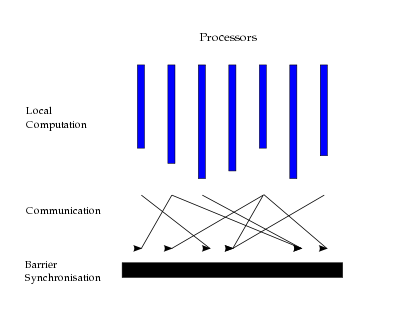
\includegraphics[width=\textwidth]{figures/bsp-model}
      \end{figure}
    \end{column}
  \end{columns}
\end{frame}

\begin{frame}
  \frametitle{Advantages \& Disadvantages}
  Advantages
  \begin{itemize}
    \item simple and easy-to-use
    \item sufficiently expressive in practice
    \item high scalability
  \end{itemize}

  \pause
  Disadvantages
  \begin{itemize}
    \item enforce users think in a vertex centric way
    \item global barrier harms performance (superstep cost determined by the slowest node)
    \item all communications happen in global space
    \item most suitable for sparse graphs
  \end{itemize}
\end{frame}

\begin{frame}
  \frametitle{Pregel's Implementation}
  \begin{itemize}
    \item master-slave runtime
    \item asynchronous communication (overlaping comm./comp.)
    \item fault tolerance (important issue on clusters)
    \item combiners as optimization
    \item aggregators as global shared state
  \end{itemize}
\end{frame}

%% \section{Pregel v.s. MapReduce}
%% \frame{\tableofcontents[currentsection]}

\begin{frame}
  \frametitle{Pregel v.s. MapReduce}
  MapReduce is another famous parallel computing framework  prior to Pregel which is also
  origined from Google. They share some design ideas such as
  \begin{itemize}
    \item BSP model
    \item high scalability
    \item master-slave runtime and fault tolerance
  \end{itemize}
  \pause
  with significant differences in other ways
  \begin{itemize}
    \item MapReduce is essentially functional while Pregel is imperative
    \item Pregel is specially designed for graph processing with domain specific knowledge \\
      Though MapReduce could also be used, it's generally ineffecient
  \end{itemize}
\end{frame}

\begin{frame}
  \frametitle{Promising Future Research}
  \begin{itemize}
    \item Graph repartioning (statically or dynamically) to elimate communication, improve locality and
      load balancing
    \item Relaxed synchronization model to improve concurrency
    \item High-level DSL and compilers enabling problem denpendent optimization
  \end{itemize}
\end{frame}

\section{Summary}
\frame{\tableofcontents[currentsection]}

\begin{frame}
  \frametitle{Summary}
  \begin{itemize}
    \item Large-scale graph and its properties
    \item Google's Pregel system: model, features, pros \&cons
    \item Some research hints
  \end{itemize}
\end{frame}

\begin{frame}
  \frametitle{References}
  \begin{itemize}
    \item Pregel: A System for Large-Scale Graph Processing, Grzegorz Malewicz et al. SIGMOD 2010.
  \end{itemize}
\end{frame}

\frame{\centerline{\Huge Q\&A}}

\end{document}
